\begin{abstract}

While invariant architectures are standard for processing symmetric data, there is growing interest in achieving invariance by applying group averaging or canonization to non-invariant backbones. However, the theoretical generalization properties of these alternative strategies remain poorly understood. We introduce a theoretical framework to analyze the generalization error of these methods by bounding their covering numbers. We establish a rigorous generalization hierarchy: the error bounds of canonized models are at best equal to the error bounds of structurally invariant and group-averaged models, and at worst equal to the bounds of non-invariant baselines. Furthermore, we show that there exist "optimal" canonizations which attain the optimal error bounds, and "poor" canonizations which attain the non-invariant error bounds, and that this depends on the regularity of the canonization.
Finally, applying this framework to permutation groups in point cloud processing, we rigorously prove that the covering number of lexicographical sorting grows exponentially with the number of points in the point cloud, whereas Hilbert curve canonization guarantees polynomial growth.
This provides the first formal theoretical justification for the empirical success of Hilbert curve serialization in state-of-the-art point cloud architectures. We conclude with experiments that support our theoretical claims. 
Our code is publicly available on \href{https://github.com/yonatansverdlov/Canonization}{GitHub}.

\end{abstract}
\section{Introduction}
The integration of geometric priors into neural networks has become a cornerstone of modern machine learning, particularly for applications involving graphs, 3D point clouds, and molecular structures. In these domains, the underlying data often exhibits inherent symmetries, meaning the target function to be learned is invariant to a specific group action. Exploiting these symmetries is known to improve sample complexity and generalization \cite{elesedy2021provably,brehmer2025doesequivariancematterscale}.

While specialized architectures, which are invariant by design, are a common method for processing symmetric data, there is growing interest in achieving invariance by applying generalized group averaging methods to non-invariant backbones.

This family of methods includes full group averaging, which is theoretically sound but intractable for all but very small groups, group augmentation, which encourages invariance by randomly sampling group transformations during training, frame averaging \cite{punyframe}, which enables invariant averaging over subsets of the group, and canonization, which maps every group orbit to a single, consistent "canonical" element.


Canonization is the most efficient of all generalized group averaging methods, as it only involves processing a single orbit representative. At the same time, it enjoys the same universal approximation guarantees as full group averaging \cite{kaba2023equivariance}. These observations have motivated researchers to define canonizations in several diverse domains. These include sign canonizations for spectral embeddings of graphs \cite{ma2023laplacian,hordan2025spectral}, canonizations of graphs \cite{lin2024equivariance} and point clouds \cite{kaba2023equivariance,pmlr-v235-baker24a,friedmann2025,zhou2026rethinkingdiffusionmodelssymmetries} including the celebrated Point Transformer V3 \cite{wu2024ptv3}, and canonization of the SMILES representation of small molecules \cite{canonicalSMILES}.


In this paper, we provide a theoretical study of canonization from the perspective of generalization. Our focus is both on comparing canonization with other options for enforcing invariance and on comparing the quality of different canonizations. Our main  contributions are threefold:

\begin{enumerate}
\item \textbf{Canonization vs. Group Averaging:} We prove that the generalization bounds of canonized models are at best equal to the bounds of group-averaged models, and at worst equal to the bounds of non-invariant models (Section \ref{sec:gen}).

\item \textbf{Canonizations and continuity:} We show that continuous, isometric canonizations attain the \emph{optimal} generalization error achieved by group averaging, while discontinuous canonizations can lead to \emph{poor} canonizations whose error bounds are identical to non-invariant models (Section \ref{sec:evaluation}).

\item \textbf{Hilbert Canonization:} We prove that
canonizing point clouds with respect to permutation via lexicographical sorting is inferior to the  Hilbert canonizations used in  Point Transformer V3 \cite{wu2024ptv3}, thus establishing the first theoretical justification for the empirical success of this method (Section \ref{sec:case_study}).
\end{enumerate}


\subsection{Related Work}
\paragraph{Canonization vs. Group Averaging} It was observed that randomized SMILES can often outperform canonized SMILES \cite{ArusPous2019,Bjerrum2017SMILESEA} (see also \cite{ito2026random}). Our first contribution gives a theoretical justification for this empirical observation.

\paragraph{Discontinuity} It was shown in \cite{dym2024equivariant,pmlr-v235-baker24a} that in many invariant learning scenarios, continuous canonizations are mathematically impossible. Attempts to mitigate this issue were made in  \cite{tahmasebi2025regularity,lin2026adaptive}. Our second contribution complements these works by showing how discontinuity of canonization hurts the generalization of the canonized model.

\paragraph{Invariance and Generalization} Many papers have considered generalization analysis of invariant models \cite{vasileiou2025survey,petrache2023approximationgeneralization,maskey2025generalization, franks2024weisfeiler}, but they do not consider canonizations. To our knowledge, the only paper considering the generalization of canonizations is \cite{tahmasebi2025generalization}. They prove that in some settings the \emph{approximation error} of canonized models is lower than group averaged models, and as a result the \emph{expected error} of canonized models can be lower when the model is presented with enough samples. In contrast, our first conclusion is that the \emph{generalization error bound} of group average models is always lower than the generalization error bound of canonized models.

\subsection{Notation}
\paragraph{Symmetry space} Throughout the paper, we will consider a metric space $(K,\rho) $, where $K$ is endowed with the action of a group $\G$. We will assume that the metric is $\G$ invariant, i.e., $ \rho(g\cdot x, g \cdot y)=\rho(x,y)$ for all $x,y\in K$ and $g \in \G $. We denote the orbit of $x\in K$ by  $[x]=\{g\cdot x| \quad g\in \G \}$, and denote the quotient space to be the space of orbits $K/\G:=\{[x]|x \in K\}$. On this space, we define a metric $\rho_\G([x],[y]):=\min_{g \in \G}\rho(g\cdot x,y)$, where we explicitly assume that the minimum in the definition of $\rho_\G$  exists, which is the case in most examples of practical interest. This assumption, together with the $\G$ invariance of $\rho$, guarantees that $\rho_{\G}$ is a metric. We call a triplet $(K,\rho,\G)$ satisfying the conditions of this paragraph a \emph{symmetry space}.

\paragraph{Canonization} Let $(K,\rho,\G) $ be a symmetry space. We say that $c:K \rightarrow K$ is a canonization if for every $x\in K$, (i) $c(x)\in [x]$, and (ii) all  $y\in [x]$ satisfy $c(y)=c(x) $. We will sometimes use canon. as an abbreviation for canonization. We also add the assumption that the canonization is Borel measurable.


\textbf{Covering number}
Let $(K,\rho)$ be a metric space, and let $A\subseteq K$. We say that $C\subseteq K$ is an $\epsilon$-cover of $A$ if, for every $x\in A$, there exists $y\in C$ such that $\rho(x,y)\leq\epsilon$. The minimum cardinality of such an $\epsilon$-cover is called the $\epsilon$-covering number of $A$ (with centers in the ambient space $K$), and is denoted by $\N(A,\rho,\epsilon)$.

\textbf{Generalization bounds via covering numbers}
Our discussion of the generalization properties of canonizations and other invariant models is based on a popular framework from \cite{xu_robustness_2012} for bounding generalization via covering numbers. We begin with a short review of this framework.

Consider the problem of learning an unknown function $f:X\to Y $ from a finite set of $n$ samples $S=\{(x_i,f(x_i)) \mid i=1,\ldots,n \}$ of the function drawn from the distribution $\mu$. Assume that we have some algorithm (e.g., gradient descent) which, given $S$, returns a hypothesis $h_S:X \to Y $. Let $\ell:Y \times Y \to \RR  $ be a function which will be used as a loss function. The \emph{expected loss} $\Lexp$ and the \emph{empirical loss} $\Lemp $ are defined via
$$\Lexp(h_S) \triangleq \mathbb{E}_{x \sim \mu} \ell(h_S(x),f(x)), \quad \Lemp(h_S)\triangleq\frac{1}{n}\sum_{i=1}^n \ell(h_S(x_i),f(x_i))$$

The \emph{generalization} error measures how much the empirical error of $h_S$ on the training data can deviate from its true loss (the expected loss) on the data distribution. It can be bounded  using the Lipschitz constants of the functions $h_S,f,\ell$ and the covering number of the domain $X$, as follows:

\begin{restatable}{theorem}{MainGeneralizationBound}
\label{thm:MainGeneralizationBound}[Proof  in Appendix \ref{app:gen}, based on \cite{xu_robustness_2012} ]
Let $(K,\rho)$ and $(Y,\rho_Y)$ be metric spaces, and assume that $X\subseteq K$ is totally bounded. Let $\mu$ be a Borel probability distribution on $X$.  Let $f:X\to Y$ be a $c_f$-Lipschitz function, let $h_S:X\to Y$ be a $c_{h_S}$-Lipschitz function, and let $\ell:Y\times Y\to[0,M]$ be a $c_\ell$-Lipschitz function. Then for any $0<\epsilon$ and $0<\delta<1$ and natural $n$,  for a training sample set $S$ generated by $n$ IID draws from  $\mu$, with probability of at least $ 1-\delta$,
$$|\Lexp(h_S) - \Lemp(h_S)| \le 2c_\ell (c_{h_S}+c_f)\epsilon+M \sqrt{\frac{2\mathcal{N}( X, \rho,\epsilon)\ln 2 + 2 \ln(1/\delta)}{n}}$$
\end{restatable}


\section{Generalization, Canonization and Group Averaging}\label{sec:gen}
In this section, we consider a task where the function  $f$ to be learned is invariant to a group action. This function is approximated by a 'learned', possibly non-invariant,  Lipschitz function $\tilde h$, which we will call the \emph{backbone model}.  We then consider three strategies of replacing  $\tilde h$ with an alternative model $h$:
\begin{enumerate}
  \item \textbf{Symmetry Agnostic models} Models that do not incorporate symmetry $h=\tilde h$.
  \item \textbf{Canonized models}  Models that incorporate symmetries by canonization, $h= \tilde h \circ c $.
  \item \textbf{Averaged and invariant models} Models that incorporate symmetries by group averaging $h(x)=\int_{\G} \tilde{h}(g\cdot x)dg $, or models where $\tilde h$ is already invariant by construction, and so $h=\tilde h $. In either case, we have that $h$ and $\tilde h$ have the same Lipschitz constant (see Proposition \ref{prop:Lavg} in the appendix).
\end{enumerate}
In this section we establish a hierarchy for the generalization bounds obtained for these three methods. The first step is the following proposition which bounds the generalization error using Theorem \ref{thm:MainGeneralizationBound}:

\begin{restatable}{proposition}{generalizationbound}[Proof  in Appendix \ref{proof_of_three_cases}]
\label{propGen}
Let $(K,\rho,\G)$ be a symmetry space. Let $(Y,\rho_Y) $ be a metric space, and assume $K$ is totally bounded. Let $\mu$ be a Borel probability distribution on $K$. Let $f:K\to Y $ be a $c_f$  Lipschitz function \textbf{which is $\G $ invariant}, and let $\ell:Y\times Y \to [0,M] $ be a $c_\ell $ Lipschitz function , then for any $0<\epsilon$ and $0<\delta<1$ and natural $n$, for a training sample set $S$ generated by $n$ IID draws from $\mu$,  with probability of at least $ 1-\delta$, we have
$$|\Lexp(h_S) - \Lemp(h_S)| \le 2c_\ell (c_{h_S}+c_f)\epsilon+M \sqrt{\frac{2\N(h_S) \ln 2 + 2 \ln(1/\delta)}{n}}$$

where
\begin{equation}\label{eq:differentN}
\N(h_S)=\threepartdef{\N(K,\rho,\epsilon)}{h_S \text{ is } c_{h_S} \text{ Lipschitz }}{\N(c(K),\rho,\epsilon)}{h_S=\tilde{h}_S\circ c, \tilde{h}_S \text { is } c_{h_S} \text{ Lipschitz, and }  c \text{ is a canon.}} {\N(K/\G,\rho_{\G},\epsilon)}{h_S \text{ is } c_{h_S} \text{ Lipschitz and  } \G \text{ invariant }}
\end{equation}
\end{restatable}

\begin{proof}[Proof idea]
The claim for a Lipschitz function $h_S$ without any invariant structure follows immediately from Theorem \ref{thm:MainGeneralizationBound}. For a canonized function  $h_S=\tilde h_{S}\circ c$, the claim follows from applying Theorem \ref{thm:MainGeneralizationBound} to the domain $X=c(K)$ and  the function $\tilde h_{S}$.
The claim for $h_S$ which is both Lipschitz and invariant follows from the fact that due to invariance $h_S, f$ can be identified with functions $\hat h_S, \hat f : K/\G \to Y $ satisfying $\hat h_S([x])=h_S(x), \hat f([x])=f(x), \forall x\in K $, and the Lipschitz constant remains unchanged after the identification.
\end{proof}


For each of the three model types considered in Proposition \ref{propGen}, a different value of $\N(h_S)$ is provided. The following simple lemma establishes the relationship between these three values:
\begin{proposition}
\label{prop:covering_bounds}
    For any symmetry space $(K,\rho,\G)$, and any $\epsilon>0$,  the following inequality holds:
    \begin{equation}
        \label{eq:coveringIneq}
        \N(K/\G,\rho_{\G},\epsilon)\leq \N(c(K),\rho,\epsilon)\leq \N(K,\rho,\epsilon)
    \end{equation}
\end{proposition}

\begin{proof}
The inequality $\N(c(K),\rho,\epsilon)\leq \N(K,\rho,\epsilon)$ is immediate since $c(K)\subseteq K$.
The inequality $\N(K/\G,\rho_{\G},\epsilon)\leq \N(c(K),\rho,\epsilon)$ follows since the quotient map $q(x)=[x]$ is $1$-Lipschitz and $q(c(K))=K/\G$. Hence, the image under $q$ of any $\epsilon$-cover of $c(K)$ is an $\epsilon$-cover of $K/\G$.

\end{proof}
Proposition \ref{propGen} and Proposition \ref{prop:covering_bounds} lead to the following conclusion:
\begin{conclusionbox}{Conclusion 1}
The generalization bounds of canonized models are at best equal to the bounds of invariant and group-averaged models, and at worst equal to the bounds of non-invariant models.
\end{conclusionbox}
Some reservations are in order: this conclusion concerns the upper bounds in Proposition \ref{propGen}, but these may not be tight. Moreover, the Lipschitz constants obtained by the different methods will not necessarily be identical. Nonetheless, these results lead us to conjecture that in terms of generalization, and overall performance, invariant and averaged models should outperform canonized models, which in turn will outperform non-invariant methods. In Section \ref{sec:experiments} we give empirical support for this claim, by providing several experiments in which group averaging outperforms canonized models. At the same time, we note that group averaging requires more computational resources and is infeasible for large groups. Invariant models also can lead to more complex and time consuming models. Thus, canonization still can have important advantages in practice. Moreover, the inequality in \eqref{eq:coveringIneq} may not be very large, in which case performance differences may be minor. The remainder of the paper focuses on this gap for different canonizations.

\section{Canonizations: From Poor to Optimal}\label{sec:evaluation}
The inequality in Equation \ref{eq:coveringIneq} gives us a theoretical way to measure the quality of a canonization. Informally, 'good canonizations' are those for which the upper bound is 'almost achieved'. Our goal in this section is to understand to what extent 'good canonizations' are possible. 

We first show that the ratio between the three different bounds in \ref{eq:coveringIneq} is at most the cardinality of the group. Thus, for small groups, the difference between canonization and invariant models is not expected to be very substantial. This is an immediate consequence from the following proposition:
\begin{restatable}{proposition}{cardinality}[See proof in ~\ref{upper_bound}]
\label{prop:cardinality}
Let $(K,\rho,\G)$ be a symmetry space, and assume $\G$ is finite. Then
\[
\N(K,\rho,\epsilon)\le |\G|\cdot \N(K/\G,\rho_{\G},\epsilon).
\]
\end{restatable}

In the next step, we will study in what cases the upper and lower bounds in \eqref{eq:coveringIneq} are achieved. Formally:
\begin{definition}
Let $(K,\rho,\G)$ be a symmetry space and let $\epsilon$ be a positive number. We say that $c$ is $(K,\epsilon) $ \emph{optimal} if it attains the lower bound in \eqref{eq:coveringIneq}, namely
$
\N(c(K),\rho,\epsilon) = \N(K/\G,\rho_{\G},\epsilon).
$
We say that $c$ is $(K,\epsilon) $ \emph{poor}  if it attains the upper bound in \eqref{eq:coveringIneq}, namely
$
\N(c(K),\rho,\epsilon)=\N(K,\rho,\epsilon).
$
\end{definition}
We will next show conditions for optimal and poor canonizations, and show how these conditions relate to the continuity of the canonization.

\textbf{Optimal canonizations:}
First, we prove that canonizations which are isometries are optimal. We say that a canonization $c:K\to K $ is an \emph{isometry} if $\rho(c(x),c(y))=\rho_{\G}([x],[y])  $ for all $x,y\in K$.
\begin{restatable}{proposition}{isometry}\label{prop:isometry}[proof in \ref{Proof_isometry}]
    Any isometric canonization $c:K\to K$ is $(K,\epsilon) $ optimal for all $\epsilon>0$.
\end{restatable}

We next use this claim to give several examples of  optimal canonizations:
\begin{restatable}{example}{isometries}\label{prop:isometries}
    The following canonizations are isometries (see proof in \ref{Proof_isometries})
\begin{enumerate}
\item The canon. $c(x)=|x|$ with respect to the action of $\{-1,1\} $ on $\R$ and the standard metric.
\item The canon. $\mathrm{sort}:\RR^n \to \RR^n $ with respect to the action of permutations and a metric $\rho$ induced by a $p$ norm.
\item The centralization canon. defined for point clouds in $\RR^{d\times n}$ with respect to the action of translation by vectors in $\RR^d$, with the metric $\rho$ induced by the Frobenius norm.
\end{enumerate}
\end{restatable}

In Proposition \ref{prop:isometryLip} in the appendix, we prove that a canonization is isometric if and only if it is $1$-Lipschitz in the standard sense.  As a result, in the setting where there can be no continuous canonizations, such as those discussed in  \cite{dym2024equivariant,pmlr-v235-baker24a}, there can be no isometric canonizations.

\textbf{Poor canonizations:} We next show that discontinuities in canonizations can lead to poor canonizations. This occurs under two conditions: firstly, the canonization is `strongly discontinuous' in the sense that it has $|\G|$ partial limits. Secondly, the domain  of the group action is chosen adversarially to exploit the discontinuity of the canonization.
\begin{restatable}{proposition}{poorcanonization}[proof in \ref{poor_proof}]
\label{prop:poor}
Let $(K,\rho,\G)$ be a symmetry space, where $\G$ is a finite group. Let $c$ be a canonization that has $|\G|$ partial limits at a point $x\in K$. Then, for any sufficiently small $\epsilon>0$, there exists a $\G$-invariant set $A\subseteq K$ such that

$$
\N(c(A),\rho,\epsilon)
=
\N(A,\rho,\epsilon)
=
|\G|\cdot \N(A/\G,\rho_{\G},\epsilon).
$$

\end{restatable}


Based on this proposition, we give two examples of poor canonizations. 

\begin{example}
\label{ex:sign_poor}
Consider the action of $\G=\{-1,1\}$ on $\R $. Consider the canonizations
$$c_1(t)=\twopartdef{|t|}{|t|>1/2}{-|t|}{|t|\leq 1/2}, \quad  c_\infty(t)=\twopartdef{|t|}{t\in \mathbb{Q}}{-|t|}{t\not \in \mathbb{Q}} $$
visualized in Figure \ref{fig:1d_canonizations}. Both of these canonizations are discontinuous and have a point with $|\G|=2 $ partial limits. Therefore, by  Proposition \ref{prop:poor} for every small enough $\epsilon>0$ we can choose an adversarial domain for which the canonization is poor. For $c_1$ we can choose for every $\epsilon\in (0,\frac{1}{2})$ the set  $K=B_\epsilon(-\frac{1}{2})\cup B_\epsilon(\frac{1}{2})$ and then $\N(K,\rho,\epsilon)=\N(c_1(K),\rho,\epsilon)=2$ and so the canonization is poor.
In the canonization $c_\infty$ the discontinuities are much more extreme. In this case, we can choose a non-adversarial domain $K=[-1,1]$, and the canonization will be poor for any $\epsilon>0$ because the covering number of a set and its closure are the same, and in our case, the closure of $c_{\infty}(K)$ will be all of $K$.
\end{example}

\begin{figure}[h]
    \centering
      \caption{\it Visualization of three canonizations for the action of $\G=\{-1,1\}$ on $\mathbb{R}$: the natural  canonization $c(x)=|x|$, which is shown to be optimal (Example \ref{prop:isometries}), and two discontinuous canonizations, which on an appropriate domain are poor (Example \ref{ex:sign_poor}).}
    \label{fig:1d_canonizations}
    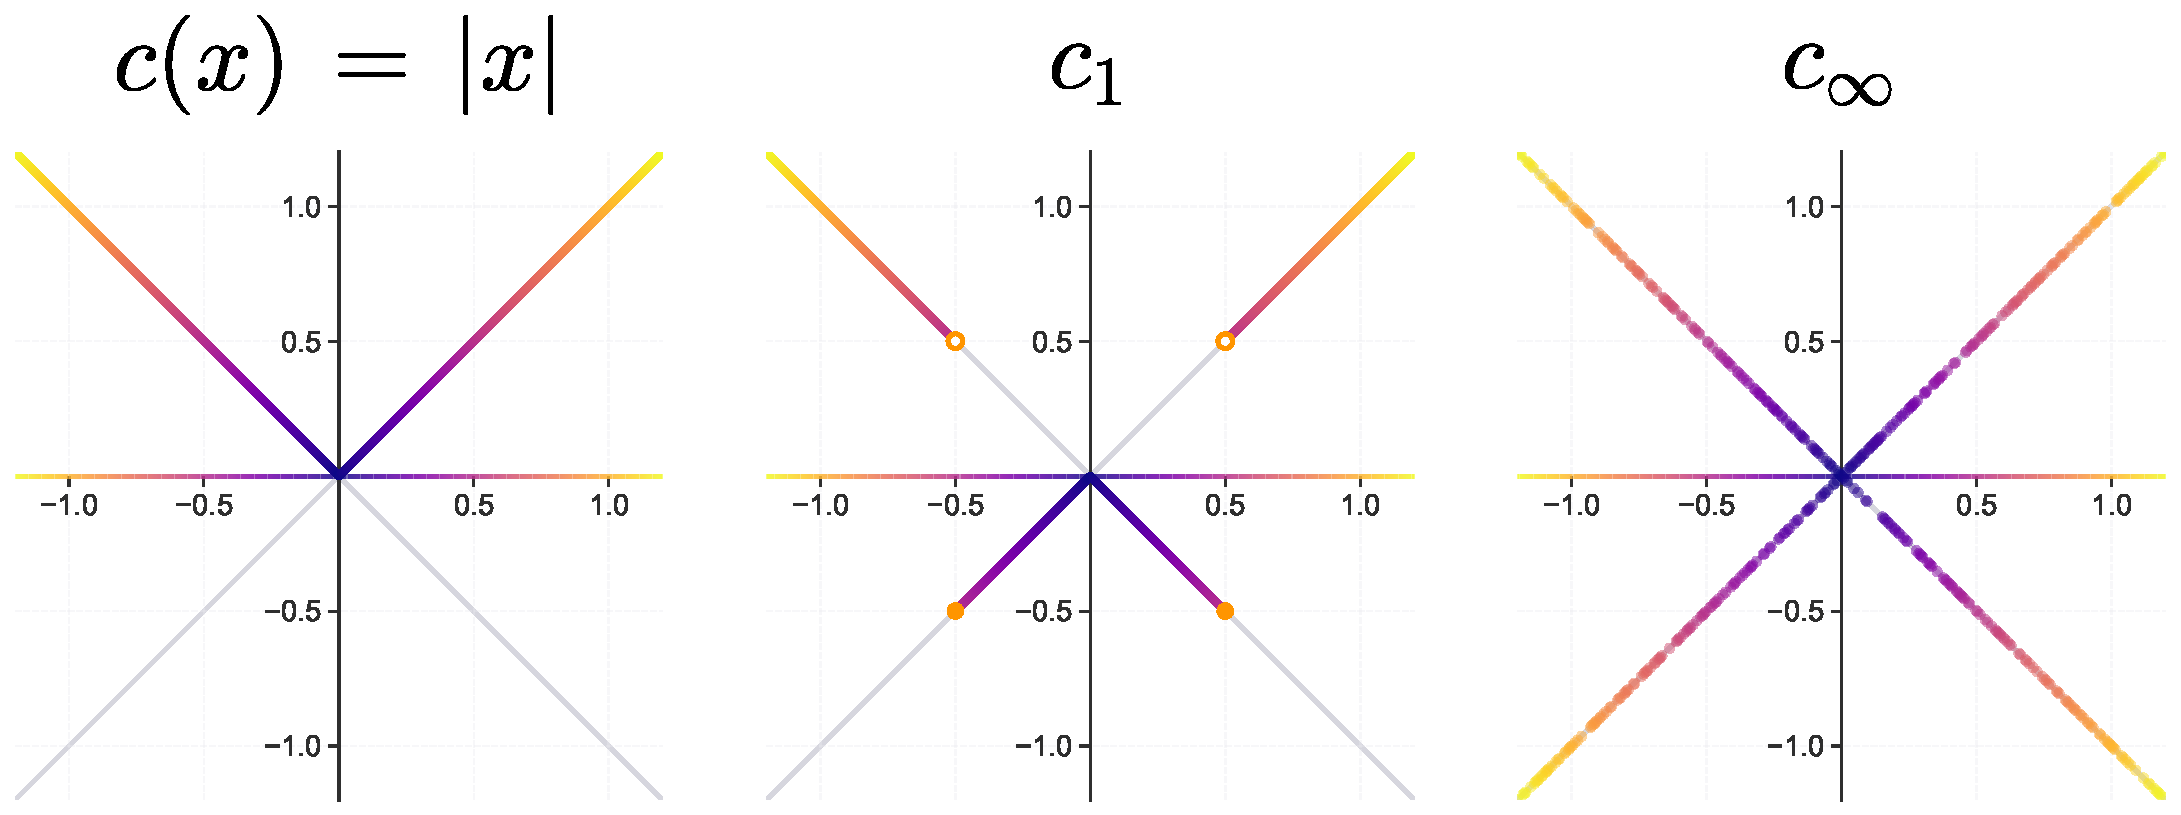
\includegraphics[width=0.8\linewidth]{figs/canonization.pdf}
\end{figure}

We next present the second example.

\begin{example}\label{ex:multisort}
Consider the action of the permutation group $\G=S_n$ on the space of matrices $\RR^{d\times n}$ by permuting the columns of the matrices. We call such matrices `point clouds'. We assume that $n,d\geq 2$ (in the case $d=1$, sorting is an isometry by Example \ref{prop:isometries}). In this case, it is known that no continuous canonization exists \cite{dym2024equivariant}. A natural (discontinuous) canonization in this scenario is lexicographical sorting $\csort$, which permutes the columns of the matrices so that the first row of the matrix is sorted from small to large, and in the event of ties in the first row, sorts according to the second row, and continues in this fashion until a permutation is uniquely defined. This canonization has $n!=|\G|$ partial limits at any matrix  $M\in \RR^{d \times n} $ satisfying that the matrix does not contain two identical columns, but $M_{1,1}=M_{1,2}=\ldots=M_{1,n}$. Thus, according to Proposition \ref{prop:poor}, for  small enough $\epsilon>0$ there exists an adversarial domain for which the canonization is poor.
\end{example}
\begin{conclusionbox}{Conclusion 2}
We show that isometric canonizations are optimal, while discontinuous canonizations can yield poor canonizations. These results give a rigorous justification for the importance of continuous canonizations.
\end{conclusionbox}


\section{Case study: Permutation Canonizations}\label{sec:case_study}

In Example \ref{ex:multisort}, we showed that lexicographical sorting is a poor canonization on an adversarial domain. In this section, we analyze the covering numbers of lexicographical sorting when considering a fixed, `natural' domain of point clouds $K=[0,1]^{d\times n}$. Throughout this section, we will consider the action of the group $\G=S_n$, and the distance induced by the element-wise infinity norm $\rho_\infty(X,Y)=\|X-Y\|_\infty $. We will show that (for fixed $\epsilon,d$) the covering number of Lexsort grows exponentially in $n$, the number of points in the point cloud, while the covering number of the quotient space only grows polynomially in $n$. Moreover, we will consider an alternative canonization based on Hilbert curves, and show that its covering numbers also grow only polynomially in $n$. The significance of this result is that it gives a theoretical justification for the choice of  Point Transformer V3 \cite{wu2024ptv3} to use Hilbert canonizations for point cloud serialization.

We begin by proving the exponential growth of Lexsort canonizations:

\begin{restatable}{lemma}{lexsortcovering}[Proof in \ref{lexsortcovering}]
\label{lem:lexsortcovering}
Let $k,d,n\geq 2$ be natural numbers, and set $\epsilon=1/(2k), K=[0,1]^{d\times n}$ and $\G=S_n$. Then the covering number of the lexicographical sorting canonization satisfies
\begin{equation}
\label{eq:exp}
\left( \frac{1}{2\epsilon}\right)^{(d-1)\cdot n + 1}\leq \N(\csort(K),\rho_\infty,\epsilon).
\end{equation}
\end{restatable}
\begin{proof}[Proof idea]
The Lexsort canonization is ineffective on the set of its `severe discontinuities'- point clouds whose first row is constant. These point clouds form a $(d-1)\cdot n+1 $ dimensional hypercube. The covering number of $\csort(K)$ is lower bounded by the covering number of this hypercube, which is the left-hand side of \eqref{eq:exp}.
\end{proof}
Next, we prove that for fixed $\epsilon,d$,  the quotient space's covering number grows polynomially in $n$:
\begin{restatable}{lemma}{quotientcovering}[Proof in \ref{quotient_cover}]
\label{lem:quotient_covering}
Let $n,d$ be natural numbers and $\epsilon\in (0,1)$. Set $K=[0,1]^{d\times n}$ and $\G=S_n$. Then the covering number of the quotient space satisfies
\begin{equation}
\label{eq:combinatorial}
\N(K/\G,\rho_{\G},\epsilon)
\leq
\binom{n+k^{d}-1}{n},
\text{ where }
k=\left\lceil \frac{1}{2\epsilon} \right\rceil .
\end{equation}
\end{restatable}
\begin{proof}[Proof idea]
Set $k=\lceil 1/(2\epsilon) \rceil $. Partition $[0,1]^d$ into $k^d$ hypercubes of side length $1/k$ and radius $1/(2k)\leq \epsilon$. Using their centers for each of the $n$ points yields an $\epsilon$-cover of $K=[0,1]^{d\times n}$. Let $C$ denote the collection of all point clouds of $n$ points whose points are centers of these hypercubes. The image of $C$ under the quotient map is  an $\epsilon$ cover $q(C)$ of $K/\G$. Note that points in $C$ which are permutations of each other are mapped by $q$ to the same orbit. Therefore, the cardinality of the cover $q(C)$ is the number of equivalence classes with respect to the relation on $C$ defined by the group: $c_1 \sim c_2 \iff \exists \tau \in S_n : c_1 = \tau\cdot c_2$. As explained in more detail in the proof, the number of equivalence classes is the combinatorial expression in \eqref{eq:combinatorial}.
\end{proof}

\subsection{Hilbert Curve Canonization}
Finally, we will provide an intuitive explanation of the Hilbert canonization and formulate the claim that its covering number exhibits only polynomial growth with respect to the number of points in the point cloud. For a full definition of the canonization and proof, see Appendix \ref{app:hilbert}.
\begin{figure}[h]
    \centering
        \caption{\it The Hilbert curves $H_m$ for $d=2$ and $m=1,2,3$ induce an ordering on a grid in $[0,1]^d $ with $2^{md}$ points. On the right, we see the discontinuous Lexsort ordering on the grid.}
    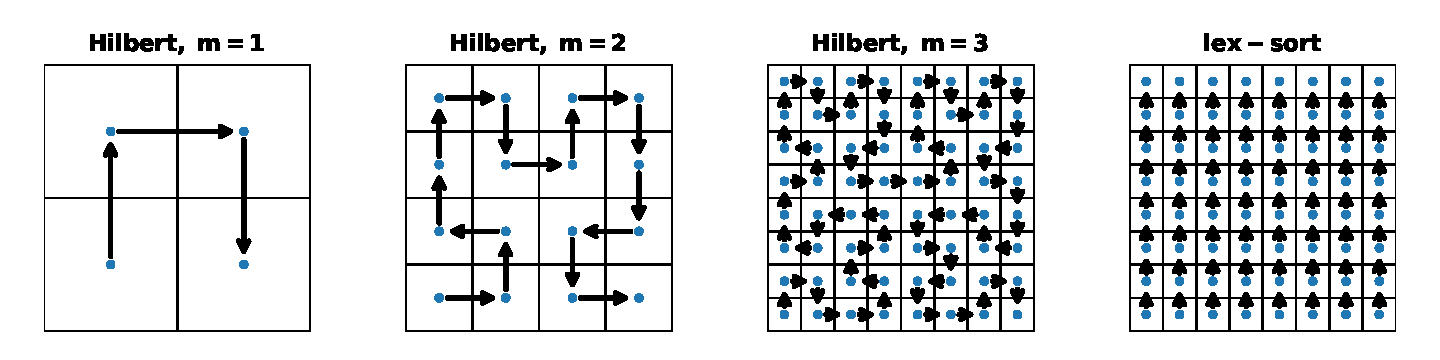
\includegraphics[width=\linewidth]{figs/hilbert_with_lex_sort.pdf}
    \label{fig:hilbert}
\end{figure}

The Hilbert curve is a space-filling curve, mapping the unit interval $[0,1]$ continuously onto a hypercube $[0,1]^d $. It is defined as a limit of curves $H_m:[0,1]\to [0,1]^d $ which are not onto but whose image becomes more and more `dense' in $[0,1]^d $ as $m$ grows, as shown in Figure \ref{fig:hilbert} for the case where $d=2$. The curves $H_m$ can be used to define an order on $[0,1]^d$ (at least on points in the image of the curve) and thus induce a canonization.
Intuitively, the advantage of this order over the Lexsort ordering is that adjacently ordered points  are mapped to nearby points in the ambient space, due to the  continuity of the Hilbert curve (see Figure \ref{fig:hilbert}).


However, while previous work \cite{wu2024ptv3,hilbertnet} cited this continuity as justification for  Hilbert ordering, a formal justification of why this continuity is important for learning has not yet been provided. We address this caveat by showing the polynomial growth of the covering number of Hilbert canonizations:
\begin{restatable}{theorem}{hilbert}[Proof in \ref{hilbert_proof}]
\label{thm:hilbert}
Let $d,n,m\geq 2$ be natural numbers, let $\epsilon\in (0,1)$, and assume that $\epsilon>2^{-m-1} $. Set $ K=[0,1]^{d\times n}$ and $\G=S_n$.    Then the covering number of the Hilbert canonization $c_m$ satisfies
$$\N(c_m(K),\rho_\infty,\epsilon)\leq  \binom{n+\lceil 1/ (2\delta) \rceil-1}{n},   \text{ where } \delta= \left(\frac{\epsilon-2^{-m-1}}{4}\right)^d$$
\end{restatable}
\begin{proof}[Proof idea]
When restricting to $n$-tuples in $K$ which are all in the image of $H_m$, the Hilbert canonization can be written as $H_m \circ \mathrm{sort} \circ H_m^{-1} $. Since $\mathrm{sort}$ (Example \ref{prop:isometries}) is an isometry, the image of $  \mathrm{sort} \circ H_m^{-1}$  can be covered efficiently. This cover can then be pushed forward to cover the image of   $H_m\circ \mathrm{sort} \circ H_m^{-1}$, using the fact that $H_m$ is Hölder continuous.
\end{proof}

 Theorem \ref{thm:hilbert} shows that the covering number of the Hilbert canonization grows at worst polynomially in $n$, for fixed $\epsilon>0$. This is in contrast with the exponential growth of the sorting canonization, proving a substantial gap between them.

\begin{conclusionbox}{Conclusion 3}
 Our analysis proves that the covering number of Hilbert canonizations is far superior to Lexsort canonization, giving a theoretical justification for its superior performance in practice.
\end{conclusionbox}

\section{Experiments}
\label{sec:experiments}
We conduct several experiments to verify our theoretical insights and their manifestation in practical learning scenarios. We focus on validating the hierarchy between group averaging, canonization, and non-invariant models (Conclusion 1), and on the hierarchy between Hilbert and Lexsort canonizations (Conclusion 3).

\paragraph{Coverage on ModelNet} In our first experiment, we considered the ModelNet \cite{wu20153d} point cloud classification task. Our first goal was to examine whether the covering-number hierarchy predicted by our theory is reflected in the geometry of real ModelNet point clouds, when comparing the quotient metric, Hilbert and Lexsort canonizations, and the original Euclidean metric.

As we do not have access to the `true point cloud' domain $K$, but only to the train and test sets, we do not compute covering numbers, but a related notion we call the coverage. For given sets $T$ (representing the test set) and $R$ (the train set), we define the coverage $\epsilon(R,T)$  to be the smallest $\epsilon$ such that $R$ is an $\epsilon$ cover of $T$. We compute the coverage by choosing, for each test sample $t\in T$, the minimum distance from $t$ to all training samples (for computational efficiency, we consider only samples with the same label as $t$). We call this number $q_t$. The coverage is then given by $\epsilon(R,T)=\max_{t\in T} q_t $. We call this measure the coverage or \emph{max coverage}. We also consider a more robust measure, the \emph{mean coverage} $\epsilon_{\mathrm{mean}}(R,T)=\mathrm{mean} \{ q_t| t\in \mathrm{Test} \} $.


\begin{table}[h]
\centering
\caption{\it Estimates of covering number on ModelNet via mean and max coverage, when using Euclidean distances, Lexsort or Hilbert canonizations, and the group distance.}
\label{tab:distances_both}
\begin{tabular}{lcccc}
\toprule
 & \multicolumn{2}{c}{\textbf{Mean coverage} $\downarrow$}
 & \multicolumn{2}{c}{\textbf{Max coverage} $\downarrow$} \\
\textbf{Method}
& \textbf{ModelNet10}
& \textbf{ModelNet40}
& \textbf{ModelNet10}
& \textbf{ModelNet40} \\
\midrule
Euclidean distance & 0.4545 & 0.3823 & 0.629  & 0.7304 \\
Lexsort distance    & 0.3770 & 0.2989 & 0.5407 & 0.5550 \\
Hilbert distance & 0.2013 & 0.1951 & 0.5283 & 0.5490 \\
Group distance   & \textbf{0.0917} & \textbf{0.0958} & \textbf{0.2742} & \textbf{0.4880} \\
\bottomrule
\end{tabular}
\end{table}

We compute the max and mean coverage on ModelNet10 and ModelNet40, using four different distances: (i) the mean pointwise Euclidean distance,  the Euclidean distance after applying (ii) Lexsort or (iii) Hilbert canonizations to the train and test sets, and (iv) the quotient metric $\rho_\G $ (in this case, the Wasserstein distance). The results, shown in Table \ref{tab:distances_both}, show that the theoretical covering number hierarchy we derived is also preserved when considering coverage of real data: the coverage of  $\rho_\G $ is the lowest, followed by Hilbert, Lexsort, and finally standard Euclidean distance.

\paragraph{Classification on ModelNet}
Next, we examine whether the hierarchy in covering numbers between the different methods translates into a corresponding hierarchy in accuracy and generalization error. We use a simple, purely non-invariant backbone, a Global MLP, and compare its performance (i) without canonization, (ii) with Lexsort canonization, and (iii) with Hilbert canonization at resolution $12$. We additionally evaluate DeepSets as an invariant Lipschitz model (exact group averaging is computationally infeasible here due to the prohibitively large permutation group). The results, shown in Table~\ref{tab:best_modelnet10and40}, reveal the expected hierarchy: Hilbert outperforms Lexsort, which in turn outperforms the plain MLP, while the invariant DeepSets model achieves the strongest overall performance. The generalization error column (defined as Train Acc.~$-$~Test Acc.) indicates that these performance differences are largely due to improved generalization.

\begin{table}[h]
\centering
\caption{\it On the ModelNet classification task, we compare a vanilla MLP without canonization, the same architecture with Lexsort and Hilbert canonization, and DeepSets as an invariant Lipschitz model. As predicted by our theory, improved invariance leads to better generalization and overall accuracy.}
\label{tab:best_modelnet10and40}
\begin{tabular}{lcccc}
\hline
 & \multicolumn{2}{c}{ModelNet10} & \multicolumn{2}{c}{ModelNet40} \\
Model & Test Acc $\uparrow$ & Gen. error $\downarrow$ & Test Acc $\uparrow$ & Gen. error $\downarrow$ \\
\hline
MLP (no canon.) & 0.573 & 0.427 & 0.441 & 0.559 \\
MLP (Lexsort)   & 0.762 & 0.215 & 0.692 & 0.256 \\
MLP (Hilbert)   & 0.782 & 0.116 & 0.742 & 0.082 \\
DeepSets        & \textbf{0.813} & \textbf{0.077} & \textbf{0.755} & \textbf{0.039} \\
\hline
\end{tabular}
\end{table}

To further verify the generality of our findings, we also trained the three Global MLP alternatives, together with DeepSets, on smaller samples from the ModelNet40 dataset. We find that the $\text{DeepSets}>\text{Hilbert}>\text{Lexsort}>\text{no canon.}$ hierarchy is preserved across all training-set sizes, as shown in Table~\ref{tab:data_scarcity} in the appendix.

We note that this experiment is only illustrative; the results attained by simple vanilla MLPs, even with Hilbert canonization, are far from state-of-the-art. In the context of our theory, this is consistent with the fact that successful models for this task are typically permutation invariant, and hence their generalization is governed by the covering number of the quotient space, which is always no larger than the covering number induced by canonization (Conclusion~1).

We next conduct further experiments to corroborate Conclusion~1, which predicts that, in terms of generalization, invariant models or group-averaged predictors should enjoy an advantage over canonized models, which in turn should improve over models that ignore the underlying invariance.

\textbf{Group averaging on PCA frames} Our first experiment is still with the ModelNet40 classification task, but while the previous experiments investigate canonization w.r.t. permutations, and implicitly rely on the fact that ModelNet models are aligned w.r.t rotations, in this experiment we use the  DeepSets \cite{zaheer2017deep} model to deal with permutation invariance, and will focus on rotation invariance: we will assume the rotational degree of freedom of point clouds in ModelNet is initially unknown, and is fixed using the PCA axes as suggested in \cite{punyframe}. Assuming the point cloud singular values are pairwise distinct, this procedure determines the point cloud orientation uniquely up to a $\{-1,1\}^3$ symmetry.

We consider four ways to deal with this symmetry: (i) Pure PCA, where the symmetry is ignored (ii) Skewness canonization, where the global sign of the $x,y$ and $z$ coordinates is chosen so that their third moment is positive (iii) group averaging and (iv) group augmentation where in each epoch a random group element is applied to the input. This  can be seen as an approximation of group averaging. The results of this experiment, detailed in Table \ref{tab:pca_canonization}  demonstrate a clear performance hierarchy. Group averaging achieves the highest overall accuracy, while group augmentation and skewness canonization yield comparable final results, with all three methods significantly outperforming the pure PCA baseline. We note that, as highlighted in Figure \ref{fig:loss_pca} in the appendix, the group augmentation approach suffers from a noticeably slower convergence rate compared to the other three methods.

\textbf{Group averaging for image classification} Next, we check our approach on image classification. We take the rotated MNIST \cite{larochelle2007empirical} dataset, and consider the action of the $p4$ group, which is the four-element group generated by $90$ degree rotations. We consider 4 approaches: simple CNN, the canonization from \cite{kaba2023equivariance} with random or learned weights (named CN(p4 frozen)-CNN and CN(p4)-CNN, respectively), and a group average over the $4$ elements of the group. As shown in Table \ref{tab:mnist}, the canonizations outperform the simple CNN, but are outperformed by group averaging, as predicted in Conclusion 1. We also see in the table that the accuracy is correlated with the mean coverage of the different methods.

\begin{table}[h]
    \centering
    \setlength{\tabcolsep}{3pt}

    \begin{minipage}[t]{0.48\linewidth}
        \centering
        \caption{\it Test accuracy on ModelNet40 with a DeepSets model with
        orientation determined by PCA, and sign ambiguity handled via averaging,
        sign augmentation, canonization, or Pure PCA (ignoring the ambiguity).}
        \label{tab:pca_canonization}

        \begin{tabular}{lc}
        \toprule
        \textbf{Method} & \textbf{Accuracy} $\uparrow$ \\
        \midrule
        Sign Averaging       & \textbf{0.760} $\pm$ 0.003 \\
        Sign Augmentation    & 0.742 $\pm$ 0.002 \\
        Skewness Canonization & 0.742 $\pm$ 0.005 \\
        Pure PCA             & 0.729 $\pm$ 0.006 \\
        \bottomrule
        \end{tabular}
    \end{minipage}%
    \hfill%
    \begin{minipage}[t]{0.48\linewidth}
        \centering
        \caption{\it Accuracy and mean coverage on Rotated-MNIST, which is
        invariant with respect to the group $p4$ of $90$ rotations. We consider
        a non-invariant CNN, two canonizations from
        \cite{kaba2023equivariance}, and group averaging.}
        \label{tab:mnist}

        \begin{tabular}{lcc}
        \toprule
        \textbf{Model} & \textbf{Test Acc.} $\uparrow$ &
        \textbf{Coverage} $\downarrow$ \\
        \midrule
         CNN               & $94.7 \pm 0.12$          & 0.185 \\
        CN(p4)-CNN        & $96.5 \pm 0.13$      & 0.175 \\
        CN(p4 frozen)-CNN & $95.5 \pm 0.15$        & 0.176 \\
        AvgCNN            & $\textbf{97.3} \pm 0.12$ & \textbf{0.167} \\
        \bottomrule
        \end{tabular}
    \end{minipage}
\end{table}


\paragraph{Canonization in deep weight spaces.}
We evaluate canonization on INR classification, where each image is represented by the weights of an implicit neural representation (INR), and the task is to predict the image class directly from these weights~\citep{pmlr-v202-navon23a}. We compare a simple MLP, a canonized MLP, and DWSNet, a specialized permutation-invariant weight-space model~\citep{pmlr-v202-navon23a}. We consider the MNIST-INR and Fashion-MNIST-INR datasets~\citep{pmlr-v202-navon23a}; details of our canonization procedure are given in Appendix~\ref{app:dws_canonization}.

For completeness, we reran the original code for the MLP and DWSNet baselines and report the results obtained from our runs. The results are shown in Table~\ref{tab:dws_canonization}. We observe that DWSNet outperforms the canonized MLP, which in turn outperforms the plain MLP, as predicted by Conclusion~1.

\begin{table}[h]
\centering
\caption{\it INR classification accuracy on MNIST and Fashion-MNIST.
We compare a non-invariant MLP,  a canonized MLP, and DWSNet, a specialized
permutation-invariant weight-space architecture.}
\label{tab:dws_canonization}
\begin{tabular}{lcc}
\toprule
\textbf{Method}
& \textbf{MNIST-INR} $\uparrow$
& \textbf{Fashion-MNIST-INR} $\uparrow$ \\
\midrule
MLP
& $16.34 \pm 0.61$
& $14.41 \pm 0.39$ \\


MLP + Canonization
& $31.06 \pm 0.46$

& $40.02 \pm 0.23$
 \\
DWSNet
& $\textbf{86.66} \pm 0.73$
& $\textbf{65.53} \pm 0.29$ \\
\bottomrule
\end{tabular}
\end{table}

\textbf{Group Averaging for Spectral Embeddings} In the Appendix
 Section \ref{sec:add_exp} we present an additional experiment showing the advantage of averaging over previously proposed canonizations, in the context of sign ambiguity present in spectral embeddings for graph learning.


\section{Conclusion}
In this paper, we establish a methodology for comparing different canonizations with group averaging
and other invariant models by studying their covering number. We show the covering number of
canonizations is at best the covering number of the quotient space (for isometric canonizations), and
at worst the covering number of the original domain (for certain discontinuous canonizations). These
results suggest that group-averaged models are preferable when computationally feasible. We also
show that the covering number of Hilbert canonizations for point clouds is substantially better than
that of Lexsort canonizations.
\paragraph{Limitations and Future Work} A limitation of our analysis is that it relies on upper bounds on
the generalization error (Proposition~\ref{propGen}), which may not be tight. Nonetheless, our experiments
indicate that lower covering numbers do correlate with better generalization and learning. Looking
towards future developments, a central contribution of this work is the demonstration that a rigorous
theoretical comparison between competing canonization methods can be established via their covering
numbers. This framework complements the traditional focus on a model’s ability to distinguish
between complex symmetric examples, instead highlighting properties that arguably exert a more
significant influence on the ultimate success of the learning process. In future work, we intend
to apply our framework to other canonizations and extend it to enable a rigorous treatment of the
generalization of frame averaging.
\begin{ack}
\textbf{Funding.} This work was supported by the Israel Science Foundation
(grant no.~272/23) and the DFG--ISF (grant no.~3597/26).

\textbf{Competing interests.} The authors declare no competing financial
interests related to this work.

N.D.\ and S.H.\ thank Jonathan W.~Siegel and Hannah Lawrence for helpful
discussions.
\end{ack}
